\chapter{Estado del Arte}
\section{Software a desarrollar}
Para tener una perspectiva más amplia y clara de lo que se pretende desarrollar, se ha realizado una búsqueda de software similar al de este proyecto,
tanto de aprendizaje musical como de otros temas que utilicen las técnicas de gamificación y de aprendizaje lúdico.

\subsection{Aplicaciones de aprendizaje}
En la actualidad existen numerosas aplicaciones en el mercado que ayudan al aprendizaje de conceptos y a la adquisición de conocimientos sobre distintos temas, 
como los idiomas, las matemáticas o el arte, entre otros. Es tan grande el auge de este tipo de herramientas que muchas de ellas están siendo
recomendadas por el colectivo docente como apoyo a los contenidos que se dan en clase. A continuación se
detallarán las aplicaciones más destacadas encontradas:

\subsubsection{Duolingo}
\begin{wrapfigure}{r}{0.2\textwidth}
    \vspace*{-0.4cm}
    \centering
    
\includegraphics[width=0.2\textwidth]{imagenes/c2/duolingo.png}
    \caption{Logo de Duolingo}
    \vspace*{-0.15cm}
\end{wrapfigure}

Duolingo es una de las aplicaciones más populares que existen para aprender idiomas. Esta aplicación se basa en el método
de aprendizaje por inmersión y en la gamificación: el usuario estudia el idioma mediante una serie de actividades lúdicas.
Aunque su principal motivación es la enseñanza de hablar y escribir en un idioma, también se incluyen actividades de
comprensión auditiva, de lectura y de vocabulario.
\newpage
La aplicación se divide en lecciones, las cuales contienen una serie de ejercicios (Figura \ref{fig:duolingo}) que el usuario debe
completar para ir avanzando por las distintas secciones.

Algunos de los ejercicios que presenta la aplicación son:
\begin{itemize}
    \item Traducción de palabras o frases con el teclado
    \item Traducción seleccionando bloques de palabras
    \item Pronunciación de palabras o frases mediante el micrófono del dispositivo
    \item Selección de imagen para el vocabulario
\end {itemize}
    Además, Duolingo ofrece en cada lección, antes de los ejercicios, una breve explicación de la gramática o vocabulario con
imágenes y definiciones sencillas, que ayudarán al usuario a entender el temario antes de comenzar la evaluación de la lección.
En cuanto al diseño, la herramienta ofrece una interfaz sencilla y fácil de usar, con botones intuitivos y coloridos que mejoran
la experiencia de usuario, algo primordial en este tipo de aplicaciones.
Por último, cabe destacar que esta aplicación es gratuita (aunque ofrece funcionalidad adicioanl de pago dentro de esta) y está disponible para dispositivos móviles (Android, iOS y Windows Phone).
\begin{figure}[H]
    \centering
    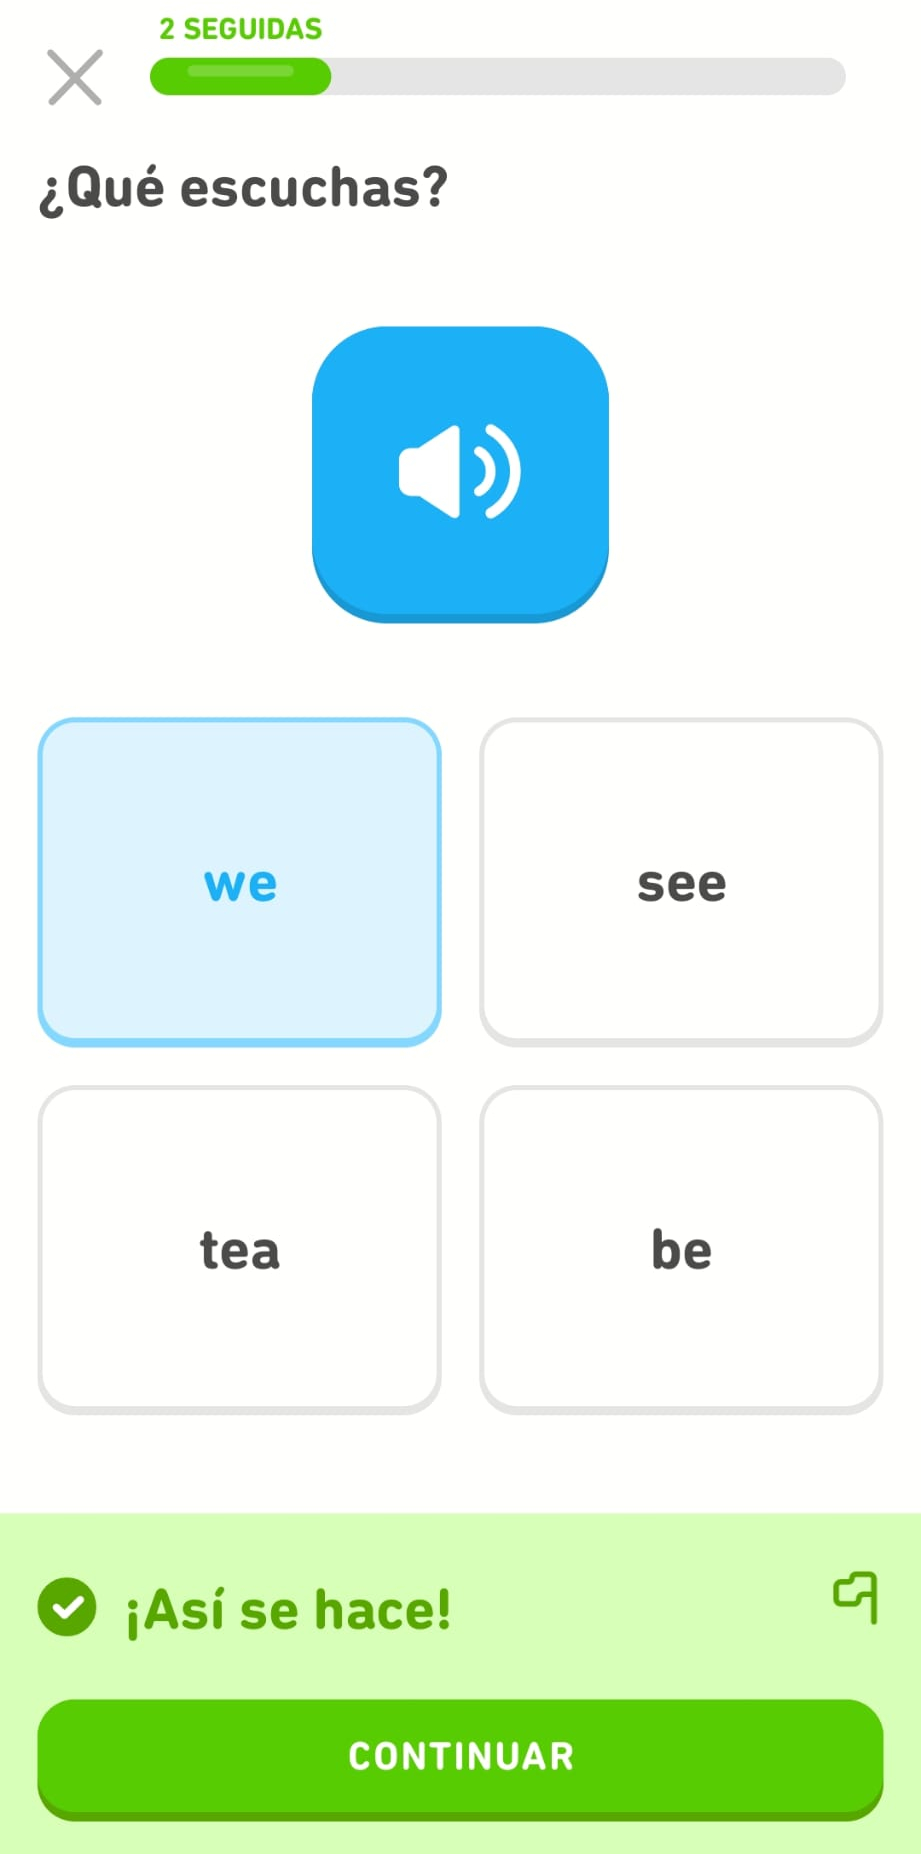
\includegraphics[width=0.33\textwidth]{imagenes/c2/duolingo.jpeg}
    \caption{Ejercicio de Duolingo donde el usuario debe adivinar qué palabra corresponde al audio}
    \label{fig:duolingo}
\end{figure} 


\subsubsection{Artly}
Artly es una aplicación móvil que permite aprender cientos de obras de arte de forma interactiva. De forma parecida a Duolingo, 
cuando el usuario abre la aplicación, se encuentra una lista de secciones (Figura \ref{fig:artly}) correspondientes a los distintos movimientos 
artísticos. Estos apartados se irán desbloqueando uno a uno a medida que el usuario vaya completando las lecciones y ejercicios.
 
En cada uno de los apartados el usuario podrá ver una lista de cuadros y esculturas de los distintos artistas que pertenecen a ese movimiento.
Al seleccionar uno de ellos, se abrirá una pantalla con la imagen del cuadro o escultura, en la que el usuario podrá ver la obra más de cerca, junto
con el título, el autor y una descripción. 
Artly incorpora además una serie de preguntas sobre las obras vistas en dicho apartado (seleccionar el autor, seleccionar el título de la obra...). 
Al finalizar las preguntas, el usuario sumará un progreso en el tema que permitirá desbloquear otros apartados y conseguir ciertos logros en su perfil.
La aplicación es gratuita pero tiene mejoras de pago que te permitirán avanzar con más facilidad y sin anuncios.

\begin{figure}[H]

    \centering
    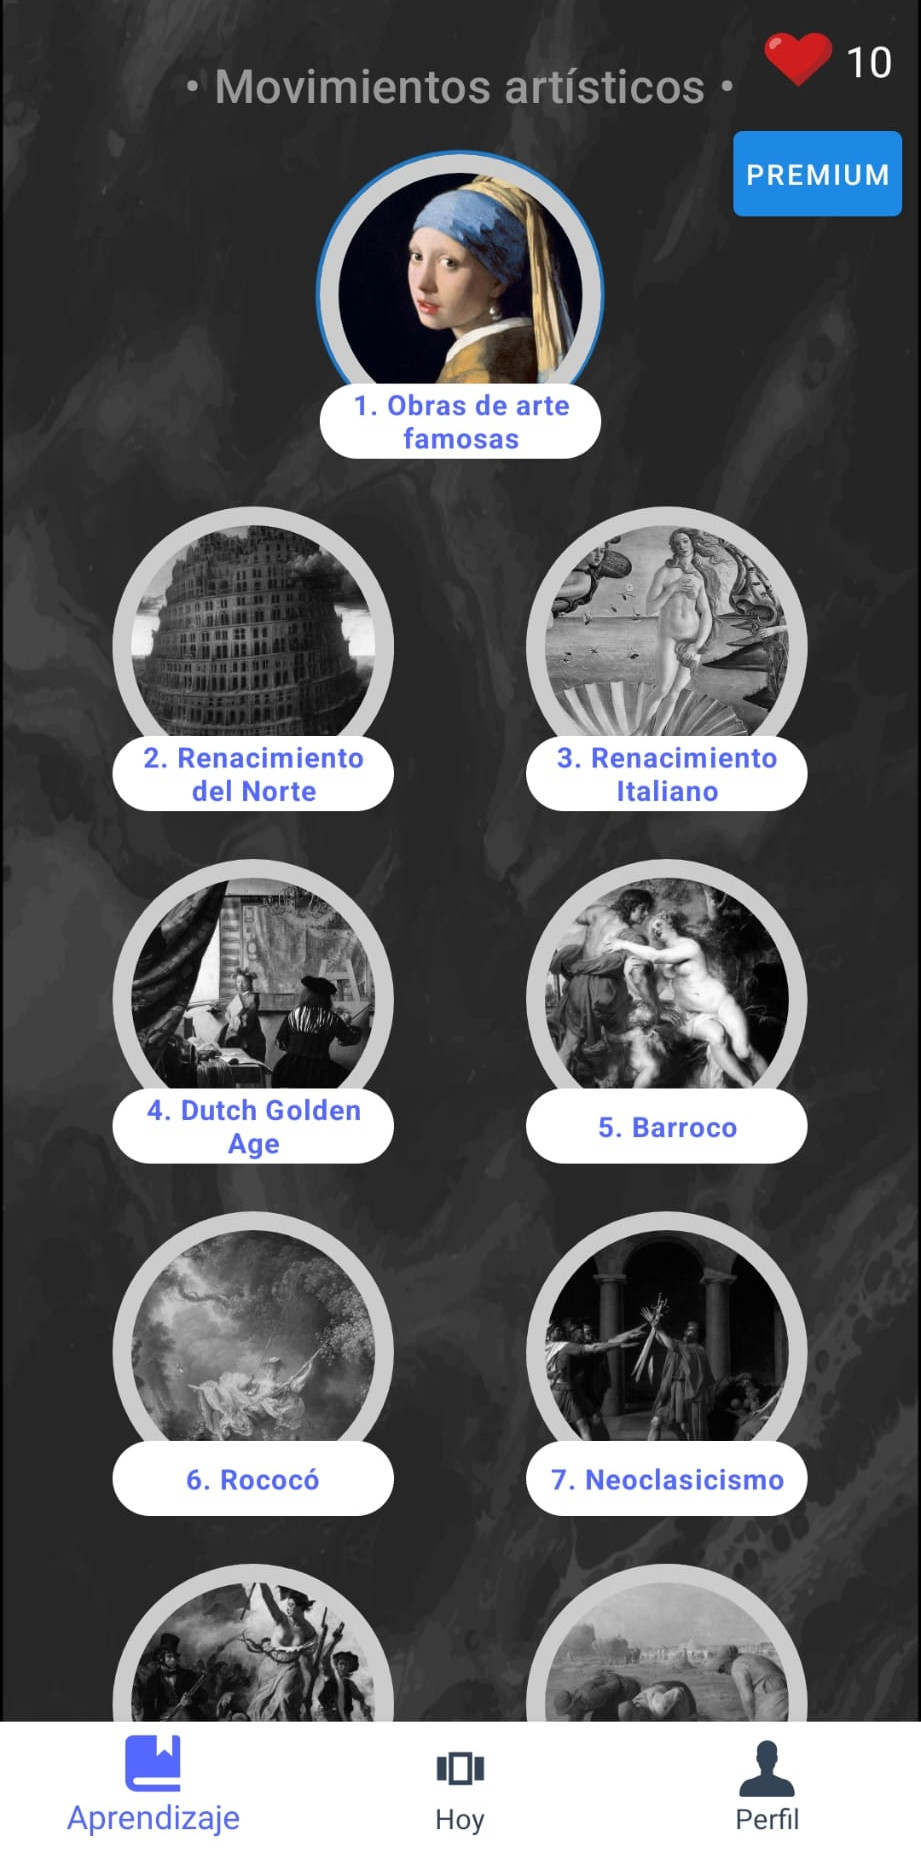
\includegraphics[width=0.4\textwidth]{imagenes/c2/artly.jpeg}
    \caption{Menú de selección de las lecciones de Artly clasificadas en movimientos artísticos}
    \label{fig:artly}

\end{figure}



\subsubsection{BMath}
BMath es un software para móviles para el aprendizaje de conceptos matemáticos mediante gamificación. Esta aplicación crea un programa personalizado para el
usuario en función del curso académico en el que esté, adaptándose a su conocimiento y a su nivel. Pese a ser gratuita, el tiempo diario que te permite el
modo básico es de 5 mintuos, mientras que si pagas te permitirá ampliarlo en 10 minutos cada día. 

Es un ejemplo de aprendizaje por gamificación ya que la aplicación es prácticamente un videojuego (de hecho, se consideran así), pues muestra una ciudad
(Figura \ref{fig:bmath}) por la que puedes mover la cámara y donde construyes distintos edificios. Para construirlos, deberás superar
una serie de pruebas sobre álgebra, geometría, etc. También obtendrás puntos de experiencia al superar los ejercicios(Figura \ref{fig:bmath2}) y, al subir de nivel, recibirás nuevos edificios y decoraciones para tu ciudad.
Con esto, se pretende que el usuario tenga la motivación de realizar ejercicios y superarlos correctamente para lograr que su ciudad.
prospere. Como alumno también puedes elegir tu propio personaje animado que te identificará en el juego.

Los diseños del software están muy cuidados y posee colores muy llamativos para que el usuario se sienta motivado y atraido. Además, la aplicación proporciona una experiencia 
de usuario agradable y motivadora, ayudando al alumno en todo momento 
a solucionar los ejercicios y enseñándole técnicas para resolverlos.

La aplicación también posee otras funciones como un apartado donde añadir recordatorios para acceder a la aplicación, preguntas para conocer cómo se siente el usuario tras cada sesión de estudio, sección parental, etc.

\begin{figure}[H]
    \centering
    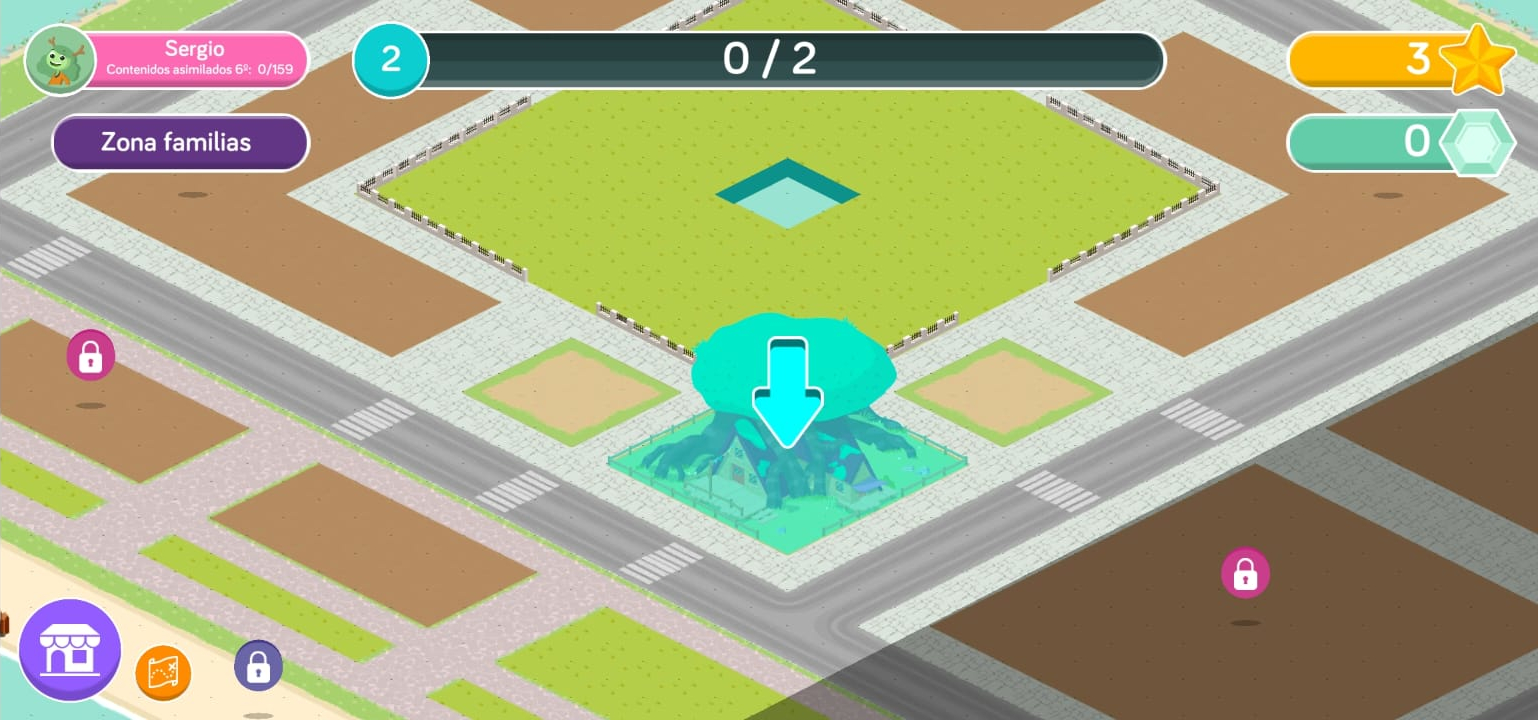
\includegraphics[width=\textwidth]{imagenes/c2/bmath.jpeg}
    \caption{Ciudad de BMath donde se seleccionan los niveles y se construyen los edificios para mostrar el progreso del usuario}
    \label{fig:bmath}

\end{figure}

\begin{figure}[H]
    \centering
    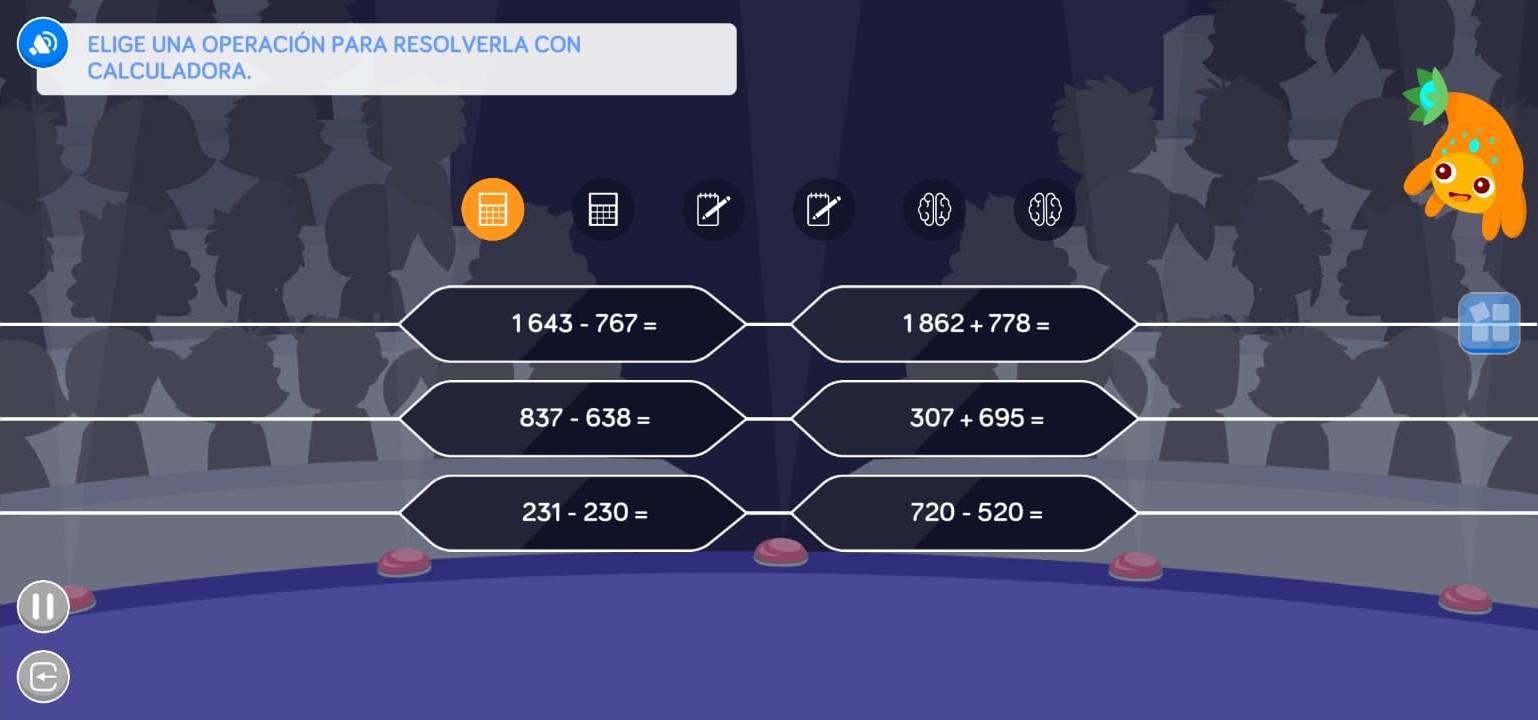
\includegraphics[width=\textwidth]{imagenes/c2/bmath2.jpeg}
    \caption{Ejercicio de BMath sobre cálculo matemático (sumas y restas) con calculadora, con papel y mentalmente}
    \label{fig:bmath2}

\end{figure}


\newpage

\subsection{Aplicaciones de aprendizaje musical}
Centrándonos ya en el tema que nos ocupa (el aprendizaje musical) existen numerosas aplicaciones que ayudan a la adquisición
de conocimientos musicales o a la ayuda a aprender a tocar un instrumento musical. A continuación se muestran algunas de ellas.


\subsubsection{Curso de Lenguaje Musical}
Esta herramienta para móvil tiene el objetivo de enseñar los conceptos básicos de lenguaje musical. La aplicación proporciona una forma de aprendizaje muy 
tradicional y que no está basada en la gamificación, ya que no dispone de ningún tipo de seguimiento del progreso ni de ejercicios para realizar sobre las lecciones aprendidas.
La app contiene una lista de lecciones (Figura \ref{fig:clm}) y cada una de ellas muestra un vídeo de un docente explicando el contenido del temario. 

Por último, en cuanto a la interfaz, la aplicación es muy sencilla y tiene un diseño poco atractivo, dando una simple lista con enlaces
a los vídeos de las lecciones sin ningún tipo de decoración o imagen.

\begin{figure}[H]
    \centering
    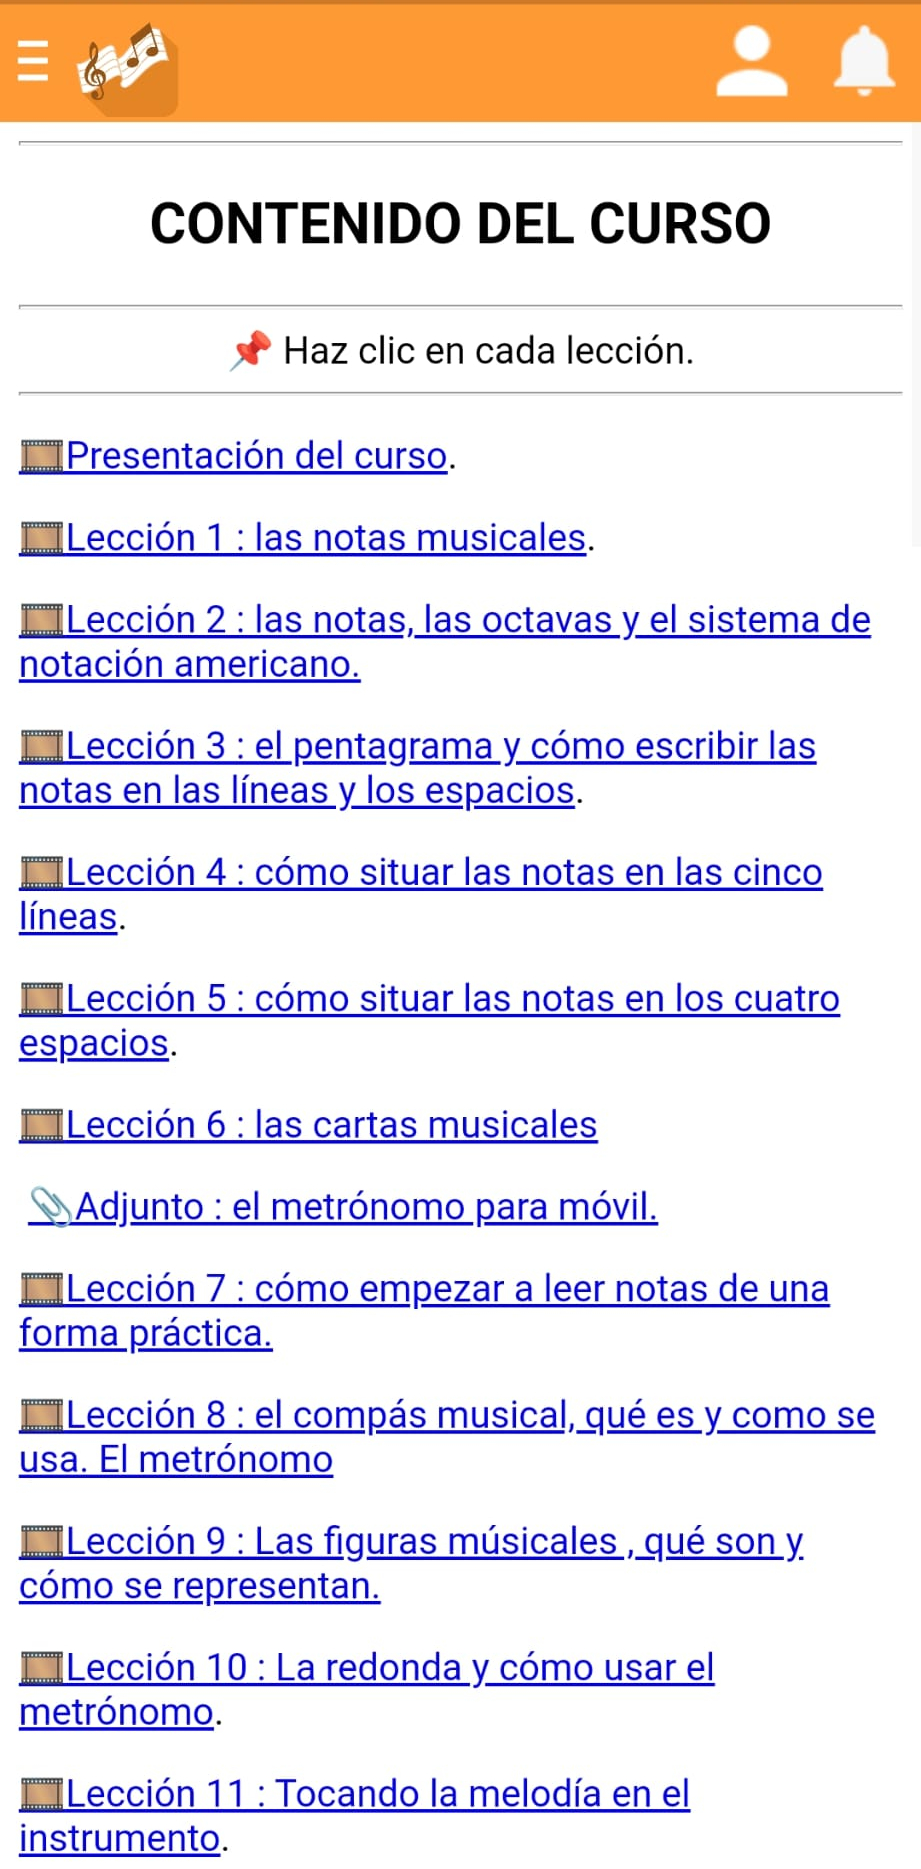
\includegraphics[width=0.4\textwidth]{imagenes/c2/cursomusica.jpeg}
    \caption{Lista de lecciones que ofrece la aplicación Curso de Lenguaje Musical}
    \label{fig:clm}
\end{figure}


\subsubsection{Sonid}
Sonid consiste en una aplicación para el aprendizaje de piano a través de la gamificación.
La aplicación se divide en distintas lecciones (Figura \ref{fig:sonid2}) que el usuario irá desbloqueando al pasarlas correctamente.
Cada lección explica unos conceptos básicos de música y piano y, al finalizar, el usuario deberá realizar una serie
de ejercicios para comprobar que ha entendido y aprendido el contenido del temario.

Algunos de los ejercicios que posee esta aplicación son:
\begin{itemize}
    \item Seleccionar la tecla en el piano que corresponde a una nota musical. (Figura \ref{fig:sonid})
    \item Responder si la tecla que se ha pulsado es una nota musical o no.
    \item Decidir qué nota musical corresponde a una tecla del piano que se ha pulsado.
\end{itemize}

Además de las lecciones, el usuario también puede practicar con escalas y acordes del piano, asi como aprenderlas en la wiki y en el diccionario que 
posee la aplicación. También dispone de un foro para que toda la gente pueda compartir sus dudas.

Por último, en cuanto al seguimiento, el usuario puede ver su progreso y sus estadísticas en su perfil, donde aparece el número de lecciones
completadas, el número de errores que ha tenido, la experiencia que tiene. Además, el usuario consigue logros al completar las lecciones y 
comparte una clasificación global con otros usuarios que también usan la aplicación.

% \subsubsection{--}

\begin{figure}[H]
    \centering
    \subfloat[\centering Ejercicio de Sonid para conocer las notas de un piano]{\label{fig:sonid}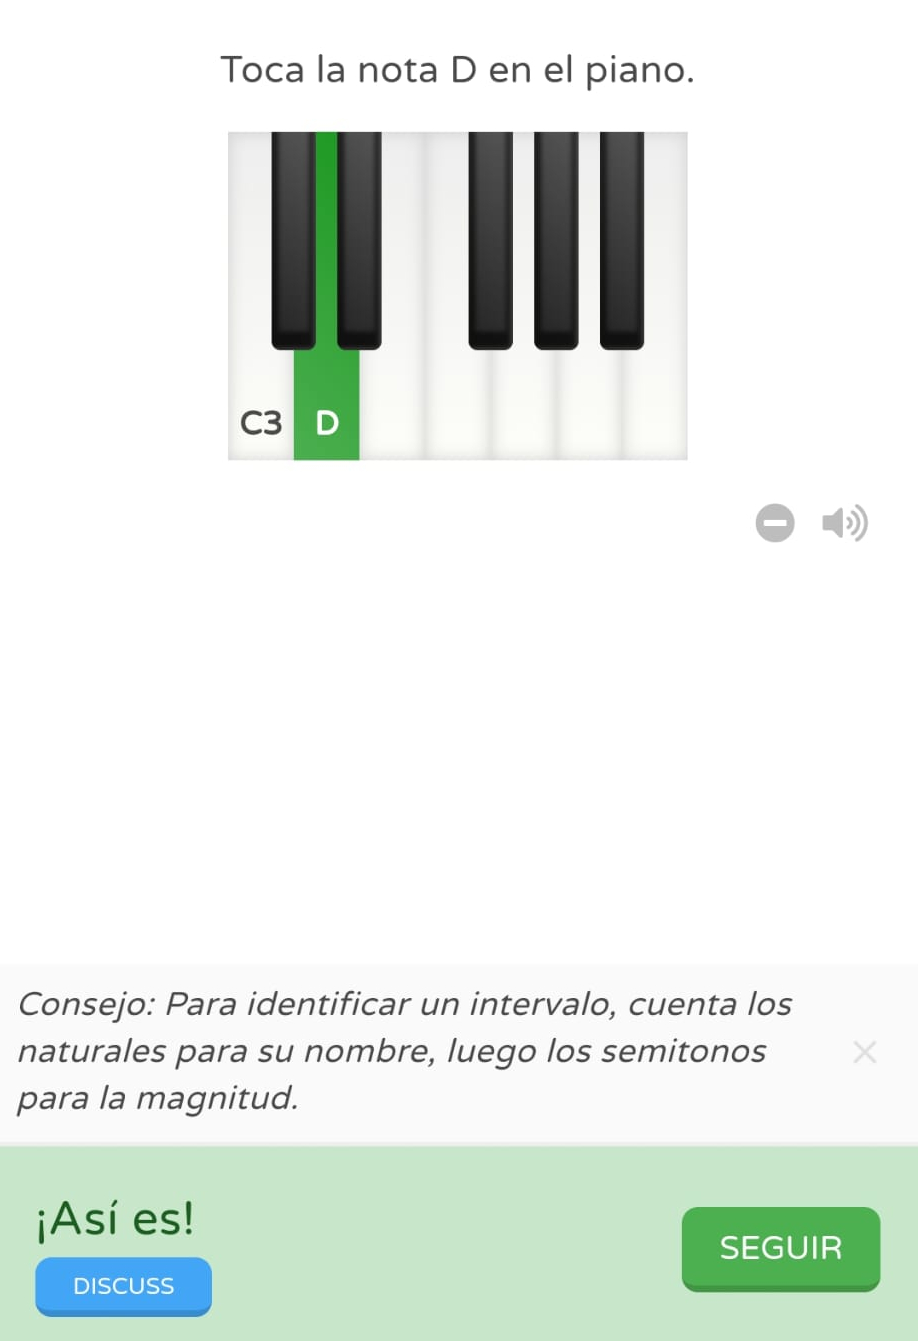
\includegraphics[width=0.35\textwidth]{imagenes/c2/sonid.jpeg}}
    \hspace{3em}
    \subfloat[\centering Menú de selección de lecciones de Sonid dividido por escalas]{\label{fig:sonid2}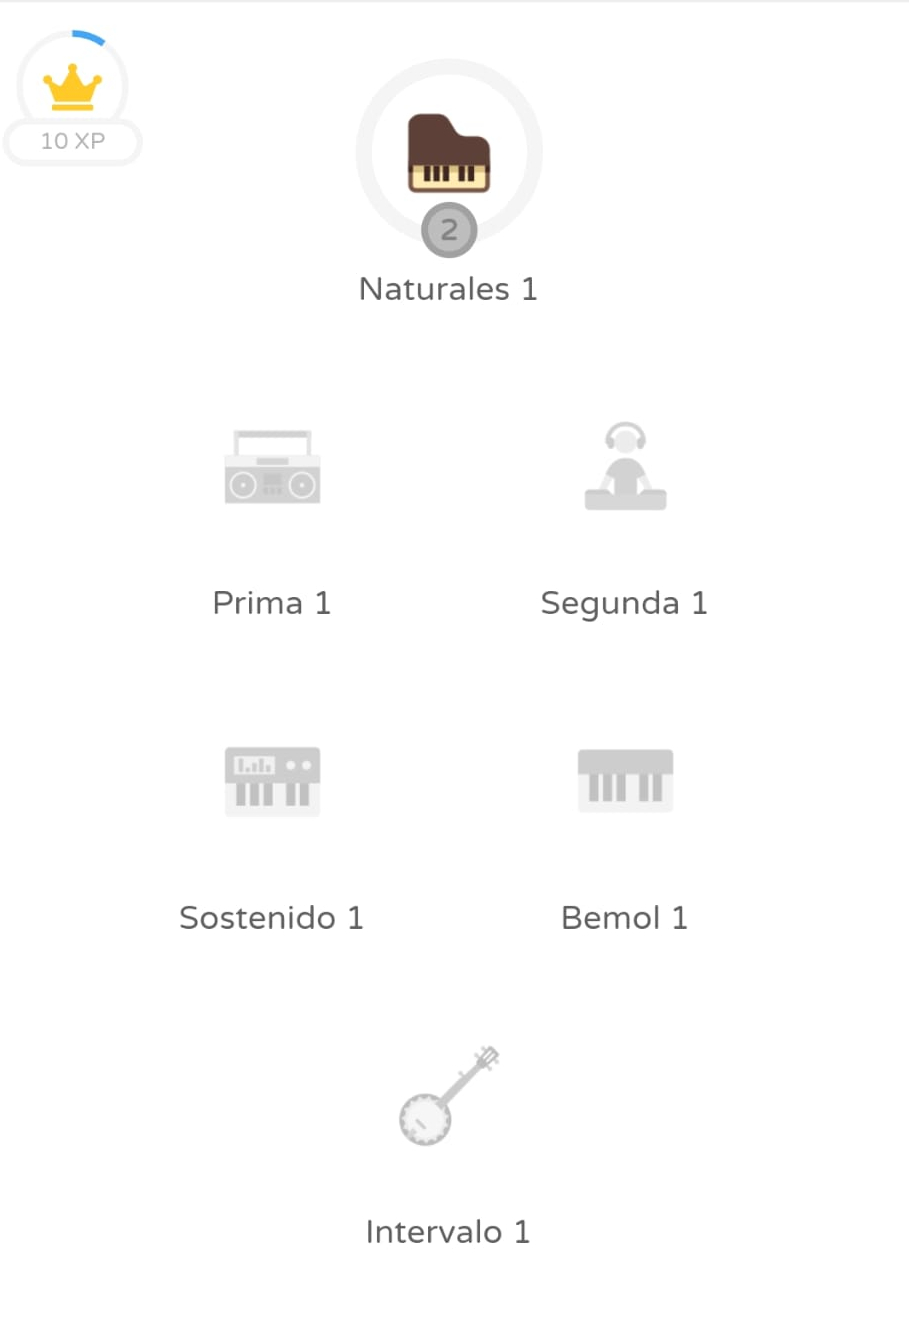
\includegraphics[width=0.35\textwidth]{imagenes/c2/sonid1.jpeg}}
\end{figure}

\newpage



\section{Desarrollo de Software}

\subsection{Flutter}
\begin{wrapfigure}{r}{0.27\textwidth}
\vspace*{-0.4cm}
\centering

\includegraphics[width=0.27\textwidth]{imagenes/c2/flutter.png}

\caption{Logo de Flutter}
\end{wrapfigure}Flutter es un kit de desarrollo software (framework) de código abierto destinado al desarrollo de aplicaciones móviles multiplataforma. Está programado en Dart, fue creado por Google y su primera versión estable se lanzó en 2018.
Se emplea para desarrollar aplicaciones para móvil, web y escritorio desde una sola base de código, lo cual permite mucha más agilidad y consistencia.

Flutter ofrece tres ventajas respecto a otros frameworks utilizados para el desarrollo de aplicaciones multiplataformas:

\begin{itemize}
\item \textbf{Compilación en nativo}
\item \textbf{Flexibilidad} para crear interfaces gráficas
\item \textbf{Desarrollo veloz}, permitiendo ver el resultado del código al instante.

\end{itemize}
Flutter está basado en el concepto de widgets, que son los elementos que componen la interfaz y la interacción del usuario. Estos widgets pueden ser modificados, añadidos o eliminados
dinámicamente, permitiendo una gran flexibilidad a la hora de crear interfaces gráficas. 

\subsection{React Native}
Framework de código abierto creado por Meta Platforms (Facebook) y destinado al desarrollo de aplicaciones muliplataforma para Android, iOS, Web, Windows, etc.
Está basado en Javascript como lenguaje de programación y en React como herramienta para la interfaz de usuario. La diferencia con React es que, en lugar de 
trabajar con el navegador, trabaja con las plataformas móviles al transformar los componentes en nativos en función de la plataforma en la que se esté
ejecutando la aplicación. 

Esta tecnología permite construir aplicaciones móviles usando solamente Javascript, con el mismo diseño que utiliza
React permitiendote realizar una interfaz de usuario completa mediante componentes. 


\begin{figure}[H]
\centering

\includegraphics[width=0.3\textwidth]{imagenes/c2/reactnative.png}
\caption{Logo de React Native}
\end{figure}


Podemos encontrar dos ventajas en este framework:

\begin{itemize}
\item \textbf{Código compartido:} tu código puede ser compartido para diferentes plataformas.
\item \textbf{Comunidad:} Existe una amplia comunidad sobre React y React Native, lo cual permite encontrar soluciones a los problemas que se puedan presentar en el desarrollo.
\end {itemize}

Como desventaja, encontramos una limitación en los componentes nativos, pues seguramente se necesite escribir algo de código
específico para un plataforma en concreto


\begin{wrapfigure}{r}{0.27\textwidth}
    \vspace*{-0.4cm}

    \centering
    
\includegraphics[width=0.27\textwidth]{imagenes/c2/dart.png}
    \caption{Logo de Dart}
\end{wrapfigure}\subsection{Dart}
Dart es un lenguaje de programación de código abierto desarrollado por Google y utilizado por Flutter.
Es orientado a objetos y de tipado estático. Surgió en 2011 como alternativa a Javascript.

Dart posee las siguientes ventajas:

\begin{itemize}
\item \textbf{Lenguaje fácil y sencillo} de aprender
\item \textbf{Acceso gratuito}
\item \textbf{Funciona en todas las plataformas}
\item \textbf{Programación estructurada y flexible}
\item Al ser \textbf{orientado a objetos}, facilita la encapsulación y reutilización de código gracias al uso de clases.
 
\end{itemize}

\subsection{Kotlin}
Kotlin es un lenguaje de programación construido sobre Java, desarrollado por JetBrains y lanzado en 2016.
Es orientado a objetos y tiene tipado estático, pero también soporta la programación por procedimientos y funciones. 

Algunas de sus ventajas son:
\begin{itemize}
\item \textbf{Compatibilidad con Java:} permite utilizar código Java en Kotlin y viceversa
\item \textbf{Lenguaje fácil y sencillo} de aprender y usar por su sintáxis similar a Java
\item \textbf{Robusto:} Es un lenguaje seguro con los valores nulos 
\item \textbf{Exactitud y claridad}: reduce el código repetido de forma sustancial y disminuye la probabilidad de error.

\end{itemize}


\subsection{NodeJS}
NodeJS es un entorno en tiempo de ejecución de código abierto, del lado del servidor y programado en Javascript. 
Es asíncrono y dirigido por eventos. Node es utilizado para el desarrollo de aplicaciones de red escalables y rápidas, ofreciendo beneficios
en rendimiento, velocidad de desarrollo, etc. 

Se utiliza en el desarrollo de aplicaciones web porque permite ejecutar Javascript del lado del servidor en lugar de en el navegador. 

Los principales motivos para utilizar NodeJS son:
\begin{itemize}
    \item \textbf{Simultaneidad de peticiones}: NodeJS es capaz de manejar múltiples peticiones al mismo tiempo gracias al modelo dirigido por eventos, 
    lo que permite una mayor escalabilidad.
    \item \textbf{Lenguaje sencillo} basado en Javascript.
    \item \textbf{Gestión de paquetes de calidad} gracias a NPM.
\end{itemize}


\subsection{React}
React es una biblioteca Javascript de código abierto que se utiliza para la creación de interfaces de usuario de forma fácil y sencilla.
Es mantenida por una gran comunidad de desarrolladores de software libre y fue lanzada en 2013. 

En React se trabaja con componentes, los cuales son elementos o partes de la interfaz de usuario que facilitarán la reutilización de código y la modularidad.

Entre las ventajas de React encontramos:
\begin{itemize}
\item \textbf{Componentes reutilizables:} React permite crear componentes que pueden ser reutilizados en otras partes de la aplicación.
\item \textbf{Fácil de aprender:} React es fácil de aprender y de utilizar, además de tener una documentación sólida y una gran cantidad de recursos online gratuitos.
\item \textbf{Rendimiento:} React es rápido y eficiente gracias al DOM virtual.
\end{itemize}

\subsection{Angular}
Angular es un framework de código abierto para el desarrollo de aplicaciones web y móviles. Está basado en TypeScript y está desarrollado por Google.
Esta tecnología también está basada en componentes, lo cual permite la creación de aplicaciones web escalables

\subsection{MongoDB}
MongoDB es una base de datos no relacional de código abierto y orientada a documentos. 
Es de tipo NoSQL, es decir, que no utiliza el modelo relacional de bases de datos tradicionales.
Cada registro de la base de datos es un documento que consta de pares clave - valor (muy similar a los objetos JSON).
Está escrito en C++ y las consultas se hacen pasando objetos JSON como parámetros.

MongoDB proporciona las siguientes ventajas:
\begin{itemize}
\item \textbf{Rendimiento:} MongoDB es más rápido porque almacena los datos directamente en un mismo sitio (colección).
\item \textbf{Simplicidad:} No hay que seguir un esquema ni unir tablas como en SQL.
\item  \textbf{Flexibilidad} para diseñar el esquema y crear las relaciones.
\end{itemize}
\begin{figure}[H]
    \centering
    
\includegraphics[width=0.4\textwidth]{imagenes/c2/mongodb.png}
    \caption{Logo de MongoDB}
\end{figure}

\subsection{Pilas MERN \& MEAN}
MERN es un conjunto de tecnologías que se utilizan para el desarrollo de aplicaciones web. Está compuesto por las siglas de MongoDB, Express (ayuda para crear y gestionar el backend en Node), React y NodeJS. MEAN es igual, pero sustituye React por
Angular. 

Hay una gran cantidad de beneficios al utilizar una de estas pilas para desarrollar una aplicación web como por ejemplo:
\begin{itemize}
\item \textbf{Cubre todo el ciclo de desarrollo}: Desde el backend hasta el frontend.
\item \textbf{Facilita el trabajo} con la arquitectura modelo-vista-controlador.
\item \textbf{Rápido desarrollo:} El desarrollo de una aplicación web con estas tecnologías es rápido y eficiente.
\item \textbf{Código abierto}: Todas las tecnologías que componen estas pilas son de código abierto y gratuitas y están respaldadas por la comunidad.
\item \textbf{Fácil mantenimiento:} El mantenimiento de una aplicación web con estas tecnologías es fácil y sencillo.
\end{itemize}

\begin{figure}[H]
    \centering
    
\includegraphics[width=0.8\textwidth]{imagenes/c2/MERN.png}
    \caption{Pilas MEAN y MERN}
\end{figure}

\subsection{MariaDB}
MariaDB es un sistema de gestión de bases de datos relacional de código abierto. Es un fork de MySQL y está desarrollado por su comunidad de usuarios. Surgió en 2009 como
consecuencia de la compra de MySQL por parte de Sun Microsystems.
Sigue un modelo relacional, lo cual significa que el contenido de los datos se almacena en tablas con un esquema más rígido que en MongoDB u otra base de datos noSQL.

Pese a haber mencionado solamente MariaDB como ejemplo de sistema de gestión de bases de datos relacional, existen muchos otros como por ejemplo PostgreSQL, MySQL, etc.


\begin{figure}[H]
    \centering
    
\includegraphics[width=0.4\textwidth]{imagenes/c2/mariadb.png}
    \caption{Logo de MariaDB}
\end{figure}